\documentclass[11pt]{article}
\usepackage[margin=1in]{geometry}
\usepackage{graphicx}
\usepackage{booktabs}
\usepackage{longtable}
\usepackage{array}
\usepackage{tabularx}
\usepackage{multirow}
\usepackage{float}
\usepackage{caption}
\usepackage{subcaption}
\usepackage{amsmath}
\usepackage{amssymb}
\usepackage{siunitx}
\usepackage{enumitem}
\usepackage{xcolor}
\usepackage{hyperref}
\usepackage{url}
\usepackage{setspace}
\usepackage{ragged2e}
\hypersetup{colorlinks=true,linkcolor=blue,urlcolor=blue,citecolor=blue}
\setlength{\emergencystretch}{3em}
\setstretch{1.08}

\title{Omori--Utsu Comparison for the Ridgecrest Interevent Period in the Fixed Mw 7.1 Fault-Zone Corridor}
\author{TRACE}
\date{}


% --- EarthLink enforced font settings (XeLaTeX) ---
\usepackage{fontspec}
\usepackage{xeCJK}
\usepackage{unicode-math}
\setmainfont{DejaVu Serif}
\setCJKmainfont{Noto Serif CJK SC}
\setmathfont{XITS Math}
\usepackage[htt]{hyphenat}
% --- end enforced font settings ---

\begin{document}
\maketitle

\begin{abstract}
This report evaluates the requested Omori--Utsu comparison for the Ridgecrest interevent period between the Mw~6.4 and Mw~7.1 mainshocks, using a fixed Mw~7.1 fault-zone corridor and its northern and southern subdivisions. The primary analysis uses events with $M \geq 3.0$ and cumulative fitting windows ending at nine prescribed periods between 0.30 and 1.404~day after the Mw~6.4 origin time. Event assignment was performed in a local metric coordinate system using the prescribed corridor geometry, then pure power-law Omori rates $\lambda(t)=K t^{-p}$ were fit by maximum likelihood with bootstrap uncertainty estimation. The fixed 35.72$^{\circ}$N split yields 109 corridor events at $M \geq 3.0$ in total, partitioned into 50 northern and 59 southern events, with clean north--south bookkeeping and no events exactly on the split line. The full corridor shows relatively stable sub-unity decay, ending at $p=0.739$ with bootstrap median 0.748 and 95\% interval [0.641, 0.860] at 1.404~day. For the primary north--south comparison, the northern and southern subdivisions are similar through the earlier cumulative windows, but from about 0.85~day onward the fitted northern $p$ values become lower than the southern values. At the final 1.404~day window, the fitted values are $p_{\mathrm{north}}=0.583$ and $p_{\mathrm{south}}=0.858$, indicating a lower late-period decay exponent in the north. However, bootstrap intervals overlap at all periods, and the magnitude of the late north--south contrast depends on the exact split latitude, so the evidence supports a moderate, not sharply resolved, inference that the northern subdivision tends to lower $p$ later in the interevent period.
\end{abstract}

\section{Scientific objective}
The scientific objective was to test whether the northern part of the fixed Mw~7.1 fault-zone corridor exhibits systematically smaller Omori decay exponents than the southern part later in the interevent period between the Mw~6.4 and Mw~7.1 Ridgecrest mainshocks. The requested primary design specified:
\begin{itemize}[leftmargin=2em]
    \item the interevent time window $(\mathrm{Mw}\,6.4,\mathrm{Mw}\,7.1)$,
    \item a fixed Mw~7.1 corridor with strike 138.0$^{\circ}$, centerline start $(-117.735813,35.897499)$, centerline end $(-117.362520,35.559488)$, and total width 6.0~km,
    \item three primary domains: entire corridor, northern area, and southern area,
    \item a primary split latitude of 35.72$^{\circ}$N, with 35.70$^{\circ}$N and 35.74$^{\circ}$N retained as robustness checks,
    \item cumulative pure power-law Omori fits,
    \item a primary magnitude threshold of $M \geq 3.0$.
\end{itemize}
The final scientific question is therefore not simply whether north and south differ at any one early time, but whether the northern subdivision becomes systematically lower in fitted $p$ than the southern subdivision in the later cumulative windows approaching the Mw~7.1 mainshock.

\section{Data products and implemented workflow}
\subsection{Input and derived analysis products}
The analysis was built from the user-specified relocated catalog and mainshock metadata, then summarized into two workflow tasks: domain preparation and Omori fitting with figures. The report relies on the concrete task outputs listed in the evidence index, especially:
\begin{itemize}[leftmargin=2em]
    \item domain diagnostics and counts from
    \url{../exp_run/outputs/01_domain_preparation},
    \item Omori fit tables, bootstrap summaries, and figures from
    \url{../exp_run/outputs/02_omori_fitting_and_figures}.
\end{itemize}

The key machine-readable files used for the report are:
\begin{itemize}[leftmargin=2em]
    \item domain count summary: \url{../exp_run/outputs/01_domain_preparation/domain_counts_primary.csv},
    \item domain metadata: \url{../exp_run/outputs/01_domain_preparation/domain_metadata.json},
    \item merged primary Omori results: \url{../exp_run/outputs/02_omori_fitting_and_figures/final_merged_primary_results.csv},
    \item primary north--south comparison table: \url{../exp_run/outputs/02_omori_fitting_and_figures/north_vs_south_primary_comparison_35p72.csv},
    \item split-sensitivity results: \url{../exp_run/outputs/02_omori_fitting_and_figures/split_sensitivity_results.csv},
    \item run metadata: \url{../exp_run/outputs/02_omori_fitting_and_figures/run_metadata.json}.
\end{itemize}

\subsection{Implemented method}
The implemented workflow follows the requested evidence chain.

\paragraph{Domain preparation.}
Interevent events were projected into a local metric coordinate system so that the prescribed Mw~7.1 centerline and its 6.0~km corridor could be represented consistently in kilometers. The saved metadata confirm the requested geometry: strike 138.0$^{\circ}$, centerline start at $(-117.735813,35.897499)$, centerline end at $(-117.362520,35.559488)$, half-width 3.0~km, and derived centerline length 50.47~km. Events within the fixed corridor were then subdivided north or south of the chosen split latitude. The primary split is 35.72$^{\circ}$N, while 35.70$^{\circ}$N and 35.74$^{\circ}$N were carried through as sensitivity tests.

\paragraph{Time reference and fitting windows.}
All times were measured relative to the Mw~6.4 origin time, with $T=0$ at 2019-07-04T17:33:49.040000+00:00. The Mw~7.1 origin time is 2019-07-06T03:19:53.040000+00:00. The cumulative comparison windows ended at the nine prescribed times: 0.30, 0.50, 0.68, 0.732, 0.85, 1.00, 1.10, 1.22, and 1.404~day. The 0.732~day marker corresponds to the M5.4 separator, and 1.404~day is the final interevent endpoint at the Mw~7.1 origin time.

\paragraph{Omori model.}
For each domain and cumulative endpoint, the primary model was the requested pure power-law rate
\begin{equation}
\lambda(t)=K t^{-p},
\end{equation}
fit by maximum likelihood using only events with $M \geq 3.0$ inside the relevant domain and before the cumulative endpoint. The implementation did not estimate a $c$ parameter. Instead, to avoid the singularity at $t=0$, each fit began at the first observed event time in that window, recorded in the results table as $t_{\min,\mathrm{used}} > 0$.

\paragraph{Uncertainty estimation.}
Bootstrap uncertainty was estimated with 1000 replicates per window. The merged results table reports the requested event counts, fitted $p$, bootstrap median $p$, and the 2.5th and 97.5th percentiles. The run metadata indicate that all 27 primary windows succeeded and that all bootstrap windows completed successfully.

\section{Domain definition and diagnostic checks}
The fixed corridor and north--south partition were established before any Omori fitting. Figure~\ref{fig:domain_diagnostic} provides the geometric diagnostic requested for the domain assignment stage. It shows the prescribed Mw~7.1 centerline and corridor boundaries, the 35.72$^{\circ}$N split line, the Mw~6.4 and Mw~7.1 mainshocks, and interevent events colored by time since the Mw~6.4 mainshock. The visual assignment is spatially coherent: events north of the split are consistently associated with the northern subdivision and events south of the split with the southern subdivision, with only limited crowding near the central boundary zone.

For the primary split at 35.72$^{\circ}$N, the saved count summary shows that the fixed corridor contains 2852 interevent events across all magnitudes, divided into 1402 northern and 1450 southern events. At the primary threshold $M \geq 3.0$, the corresponding counts are 109 total, 50 northern, and 59 southern. The compact context further states that the integrity checks show exact additivity of north plus south to the full corridor and no event lying exactly on the split line, indicating a clean non-overlapping partition.

\begin{figure}[H]
    \centering
    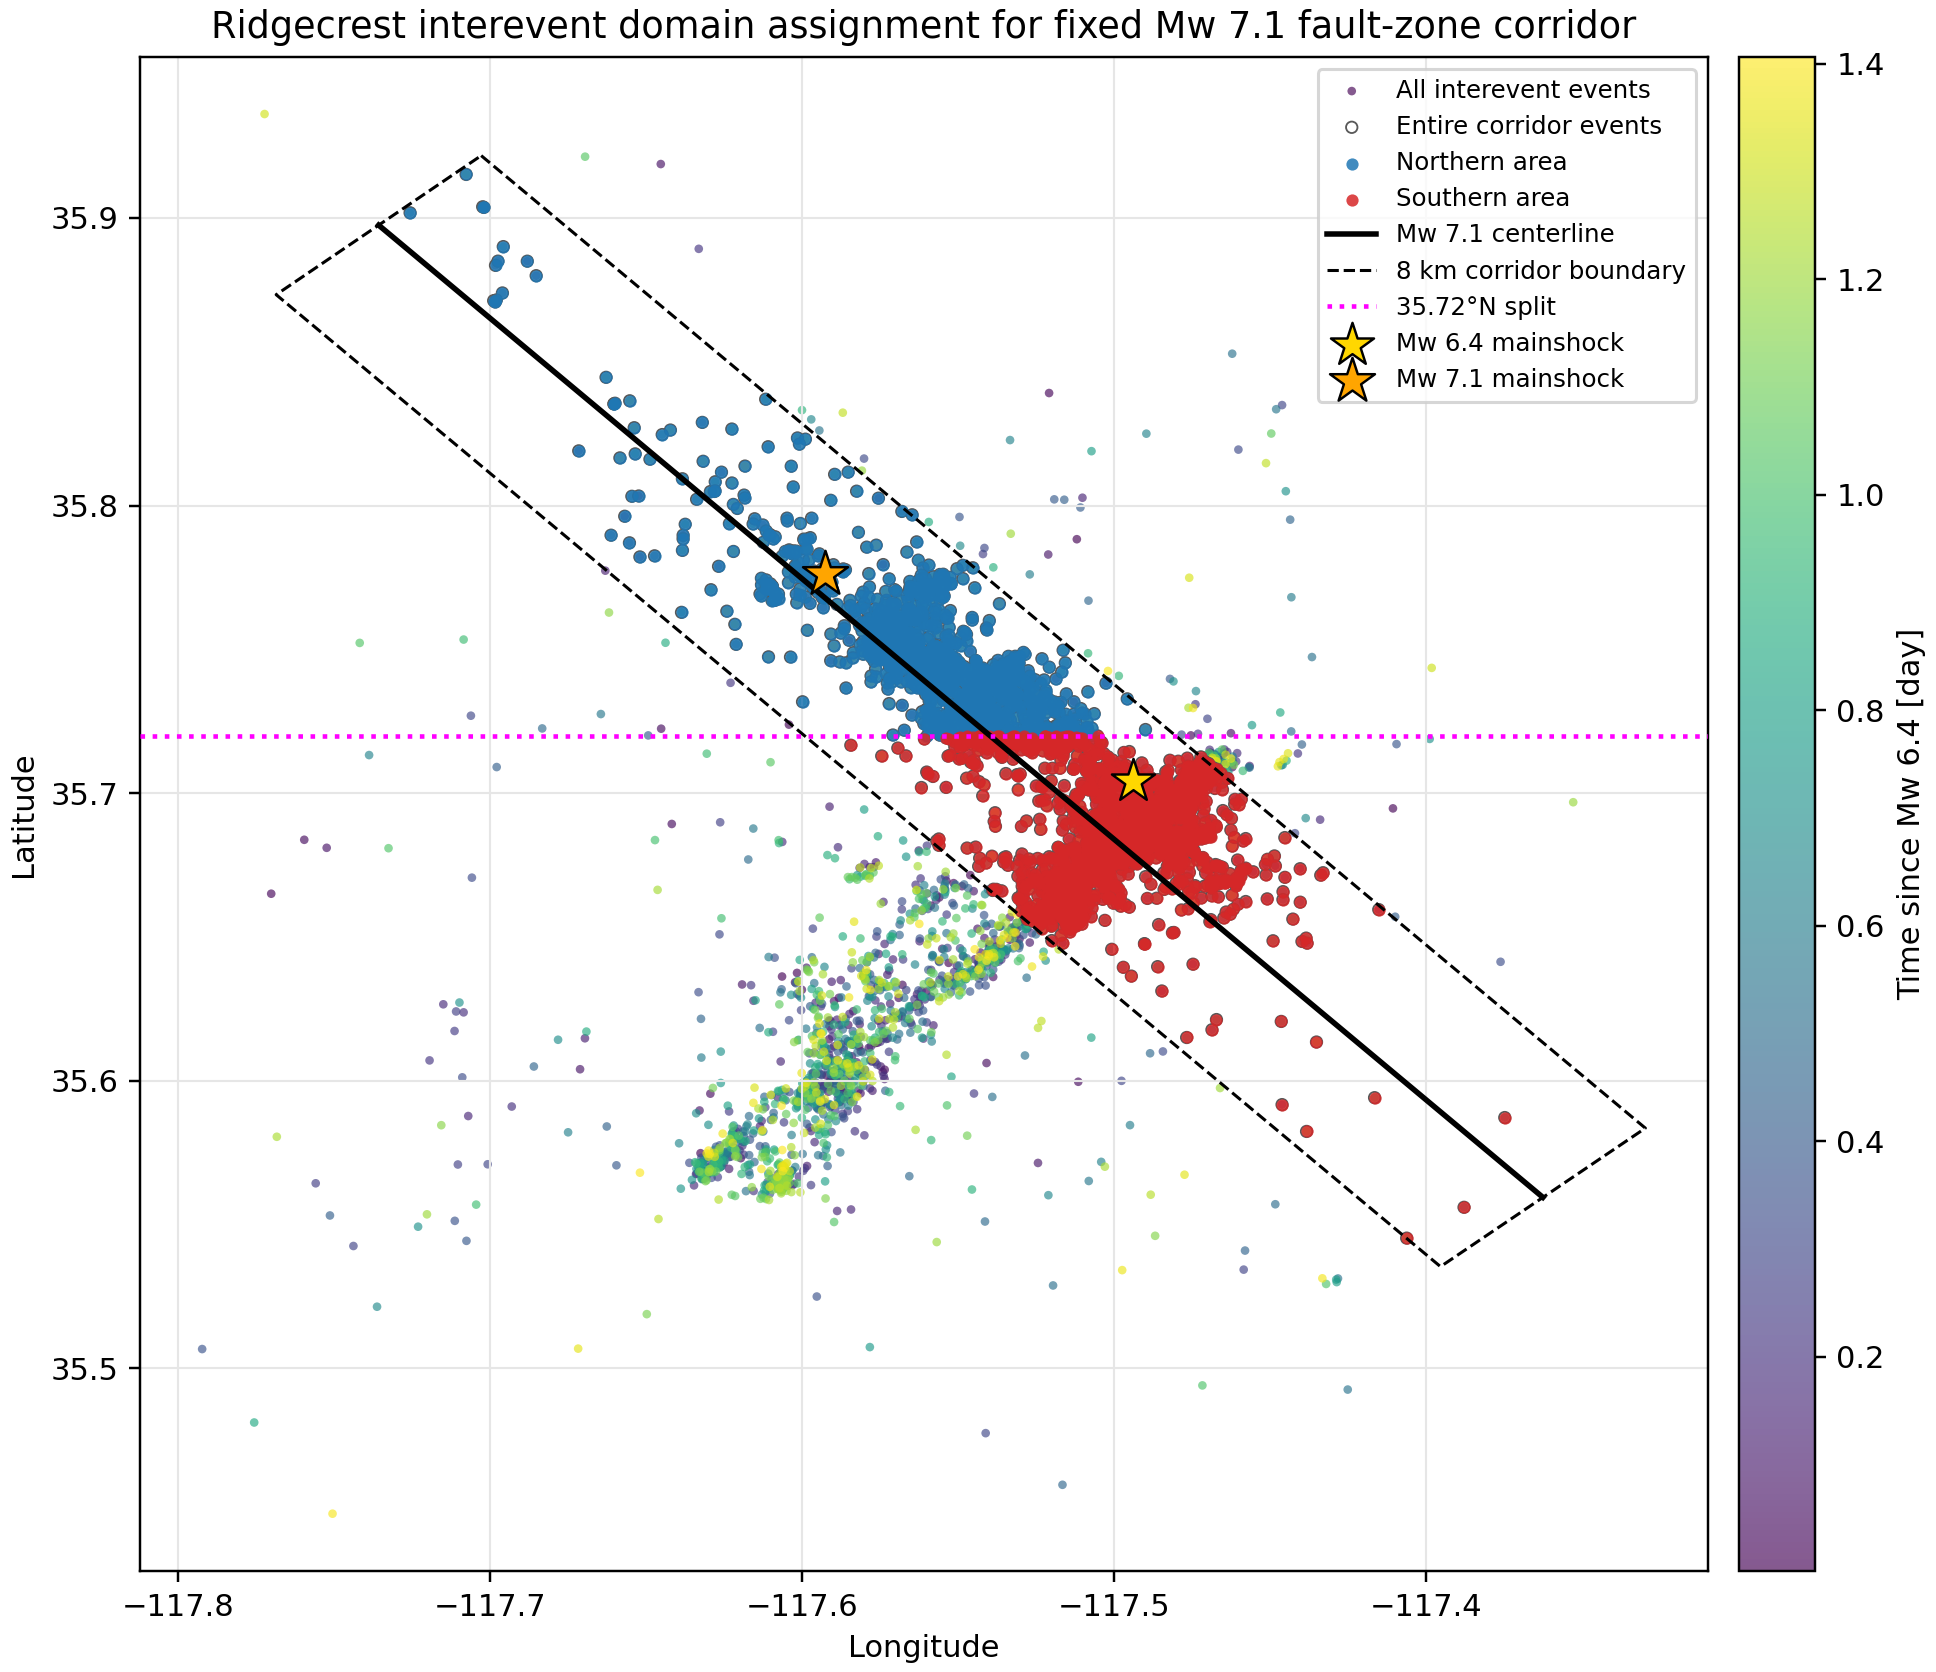
\includegraphics[width=0.88\textwidth]{../exp_run/outputs/01_domain_preparation/domain_assignment_diagnostic.png}
    \caption{Domain-assignment diagnostic for the fixed Mw~7.1 fault-zone corridor. The figure shows the prescribed corridor centerline and 6~km width, the primary 35.72$^{\circ}$N split line, the two mainshocks, and interevent seismicity colored by time since the Mw~6.4 mainshock. Events assigned to the northern and southern subdivisions are spatially separated in a visually consistent way, supporting the geometric domain construction used in the Omori analysis.}
    \label{fig:domain_diagnostic}
\end{figure}

\begin{table}[H]
\centering
\caption{Primary domain counts for the fixed 35.72$^{\circ}$N partition, from the saved count summary.}
\label{tab:domain_counts}
\begin{tabular}{lrrr}
\toprule
Domain & Split latitude ($^{\circ}$N) & Interevent count (all $M$) & Count for $M \geq 3.0$ \\
\midrule
Entire area & 35.72 & 2852 & 109 \\
Northern area & 35.72 & 1402 & 50 \\
Southern area & 35.72 & 1450 & 59 \\
\bottomrule
\end{tabular}
\end{table}

\section{Primary Omori comparison results}
\subsection{Main figure and overall behavior}
The primary comparison is summarized in Figure~\ref{fig:main_figure}. Panel~a shows fitted $p$ values against cumulative period for the entire corridor, northern subdivision, and southern subdivision, with bootstrap uncertainty bars. Panel~b shows the observed whole-corridor seismicity-rate decay on log--log axes for the final 1.404~day window, together with the fitted pure power-law curve.

The main figure supports three first-order observations. First, the entire corridor remains in a relatively stable sub-unity regime, with $p$ mostly between about 0.70 and 0.81 across the cumulative windows. Second, the southern subdivision is also stable, with fitted $p$ remaining near 0.79--0.86 through most of the interevent period. Third, the northern subdivision changes more strongly with time: it begins near $p\approx 0.98$ in the earliest 0.30~day window, becomes similar to the south through about 0.68--0.732~day, and then drops below the south from 0.85~day onward. The earliest northern point is plotted as a low-count open-circle case because $N=19 \leq 20$, exactly as requested.

\begin{figure}[H]
    \centering
    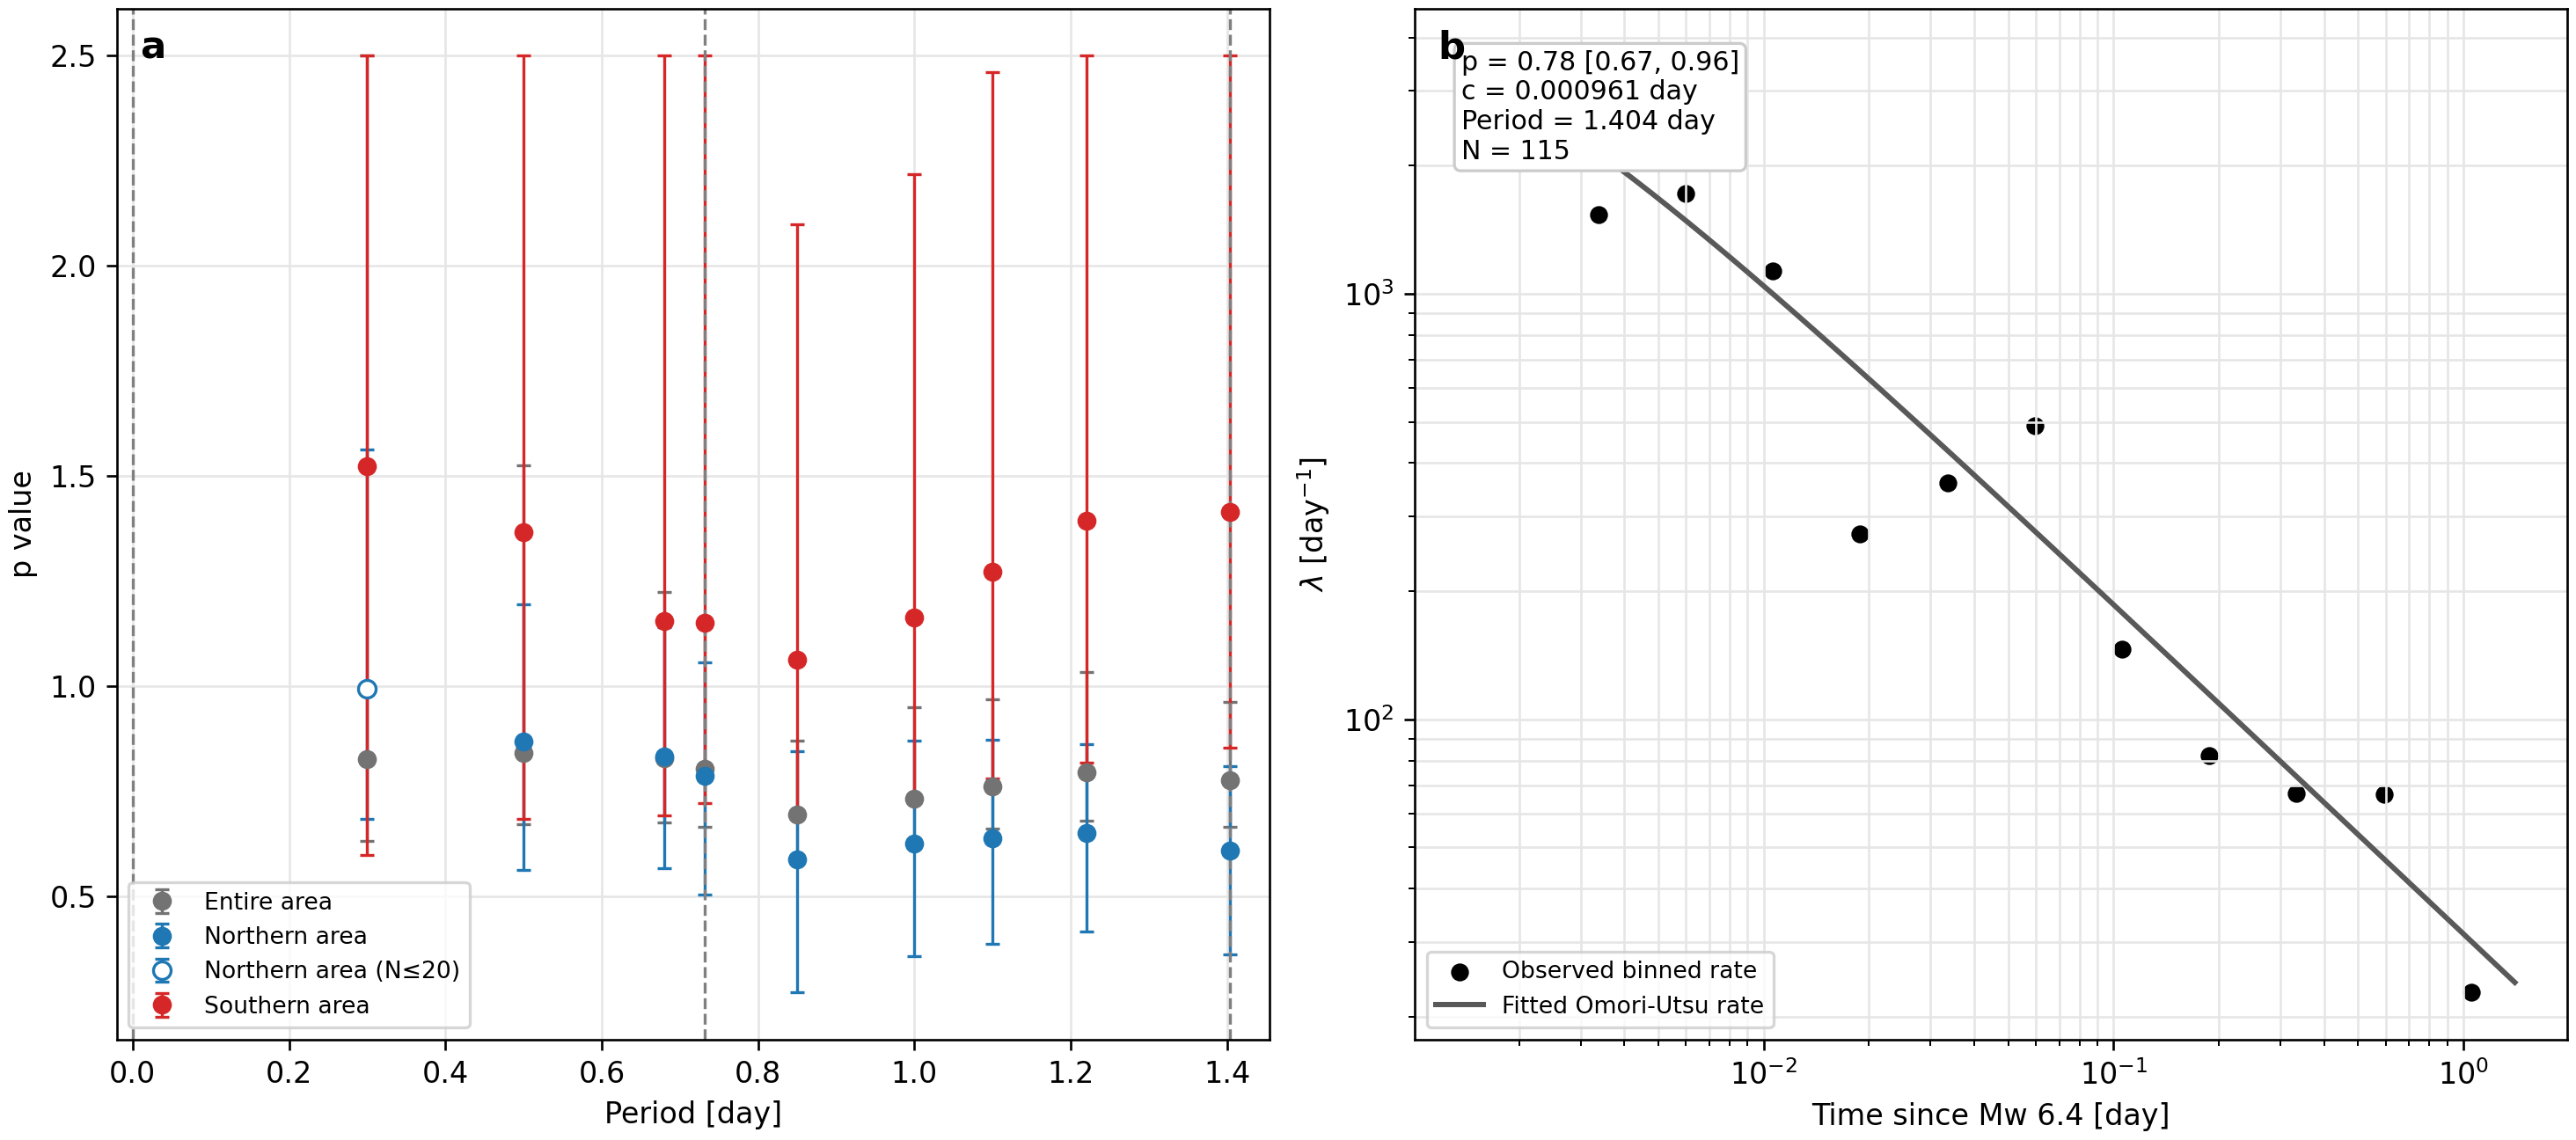
\includegraphics[width=0.92\textwidth]{../exp_run/outputs/02_omori_fitting_and_figures/main_two_panel_omori_comparison.png}
    \caption{Primary Omori comparison. Panel~a shows cumulative pure power-law estimates of the decay exponent $p$ for the entire corridor (gray), northern area (blue), and southern area (red) using the primary 35.72$^{\circ}$N split and $M \geq 3.0$. The northern 0.30~day point is an open blue circle because $N\leq 20$. Vertical reference lines mark the start, the 0.732~day M5.4 separator, and the final 1.404~day interevent endpoint. Panel~b shows the observed whole-corridor seismicity rate versus time since Mw~6.4 on log--log axes for the final cumulative window, together with the fitted power-law curve; the figure annotation reports $p=0.74$ with bootstrap interval [0.64, 0.86] and $N=106$.}
    \label{fig:main_figure}
\end{figure}

\subsection{Numerical summary of the primary 35.72$^{\circ}$ split}
Table~\ref{tab:primary_results} summarizes the principal fitted and bootstrap quantities for the nine cumulative windows in the three primary domains. All 27 primary windows are marked successful in the merged results file.

Several features are numerically clear:
\begin{enumerate}[leftmargin=2em]
    \item \textbf{Entire corridor:} the fitted $p$ values remain within a narrow range of 0.696--0.811 for the first eight windows and end at 0.739 for the 1.404~day window. The corresponding bootstrap median at 1.404~day is 0.748 with a 95\% interval of [0.641, 0.860].
    \item \textbf{Northern area:} fitted $p$ decreases from 0.976 at 0.30~day to 0.787 at 0.732~day, then drops to 0.567 at 0.85~day and remains low through the final period, ending at 0.583. The bootstrap median at 1.404~day is 0.581 with interval [0.319, 0.790].
    \item \textbf{Southern area:} fitted $p$ is comparatively steady, ranging from 0.713 in the earliest window to 0.858 at the final period, with the late cumulative windows concentrated near 0.80--0.86. The 1.404~day bootstrap median is 0.849 with interval [0.703, 0.982].
\end{enumerate}

\begin{table}[H]
\centering
\caption{Primary cumulative Omori results for the fixed 35.72$^{\circ}$N partition and $M \geq 3.0$, summarized from the merged primary results file. Values are fitted $p$ followed by bootstrap median and 95\% interval in parentheses.}
\label{tab:primary_results}
\small
\begin{tabular}{>{\RaggedRight\arraybackslash}p{1.5cm} >{\RaggedLeft\arraybackslash}p{3.7cm} >{\RaggedLeft\arraybackslash}p{3.7cm} >{\RaggedLeft\arraybackslash}p{3.7cm}}
\toprule
Period (day) & Entire area & Northern area & Southern area \\
\midrule
0.30 & 0.770 (0.790 [0.639, 0.957]), $N=65$ & 0.976 (1.017 [0.635, 1.399]), $N=19$ & 0.713 (0.733 [0.542, 0.919]), $N=46$ \\
0.50 & 0.811 (0.822 [0.683, 0.970]), $N=72$ & 0.862 (0.868 [0.531, 1.175]), $N=24$ & 0.791 (0.802 [0.630, 0.976]), $N=48$ \\
0.68 & 0.785 (0.802 [0.671, 0.935]), $N=80$ & 0.801 (0.817 [0.500, 1.102]), $N=27$ & 0.794 (0.813 [0.664, 0.963]), $N=53$ \\
0.732 & 0.787 (0.806 [0.675, 0.930]), $N=83$ & 0.787 (0.795 [0.487, 1.052]), $N=29$ & 0.799 (0.817 [0.657, 0.964]), $N=54$ \\
0.85 & 0.696 (0.712 [0.572, 0.830]), $N=96$ & 0.567 (0.566 [0.229, 0.823]), $N=39$ & 0.785 (0.806 [0.665, 0.955]), $N=57$ \\
1.00 & 0.717 (0.721 [0.602, 0.835]), $N=98$ & 0.579 (0.566 [0.252, 0.831]), $N=40$ & 0.805 (0.813 [0.679, 0.953]), $N=58$ \\
1.10 & 0.733 (0.736 [0.612, 0.848]), $N=99$ & 0.611 (0.596 [0.301, 0.838]), $N=41$ & 0.805 (0.817 [0.678, 0.954]), $N=58$ \\
1.22 & 0.766 (0.763 [0.621, 0.882]), $N=100$ & 0.648 (0.628 [0.347, 0.839]), $N=42$ & 0.805 (0.812 [0.677, 0.949]), $N=58$ \\
1.404 & 0.739 (0.748 [0.641, 0.860]), $N=106$ & 0.583 (0.581 [0.319, 0.790]), $N=47$ & 0.858 (0.849 [0.703, 0.982]), $N=59$ \\
\bottomrule
\end{tabular}
\end{table}

\subsection{Direct answer to the scientific question}
The direct north--south comparison file for the primary 35.72$^{\circ}$ split shows that the north does \emph{not} remain lower than the south throughout the whole interevent period. Instead, the pattern is temporal:
\begin{itemize}[leftmargin=2em]
    \item At 0.30~day, the fitted north value exceeds the south value ($0.976$ versus $0.713$; difference $+0.263$).
    \item From 0.50 to 0.732~day, the two series are very similar, and the fitted difference shrinks to near zero by 0.68--0.732~day.
    \item From 0.85~day onward, the fitted northern series becomes consistently lower than the southern series. The fitted north-minus-south differences are $-0.218$ at 0.85~day, $-0.226$ at 1.00~day, $-0.193$ at 1.10~day, $-0.156$ at 1.22~day, and $-0.274$ at 1.404~day.
\end{itemize}

Therefore, the requested later-period tendency is present in the fitted values: in the later cumulative windows, the northern subdivision does show systematically smaller $p$ than the southern subdivision. However, the same comparison table indicates that the bootstrap interval-overlap flag remains true for every period, including the later windows. This means the late north-lower-than-south pattern is qualitatively persistent but not strongly separated in uncertainty space.

\section{Late-period interpretation and robustness}
\subsection{Interpretation of the later cumulative windows}
For the primary 35.72$^{\circ}$ split, the later cumulative windows beginning at 1.10~day are explicitly flagged as later-period windows in the comparison table. In these windows, the northern fitted $p$ values stay below the southern values by approximately 0.16--0.27. By the final 1.404~day period, the contrast is substantial in point-estimate terms: $p_{\mathrm{north}}=0.583$ and $p_{\mathrm{south}}=0.858$.

Interpreted within the requested pure power-law model, a smaller $p$ indicates slower temporal decay of activity with increasing time. The late interevent northern subdivision therefore appears to retain comparatively more persistent activity than the southern subdivision. Because this interpretation rests on cumulative windows, it summarizes the integrated behavior of all prior activity up to each endpoint rather than a sequence of disjoint intervals.

\subsection{Split-line sensitivity}
The robustness test using 35.70$^{\circ}$N, 35.72$^{\circ}$N, and 35.74$^{\circ}$N shows that the sign of the later north--south contrast is fairly stable, while its magnitude changes with the exact split latitude.

At the final 1.404~day window:
\begin{itemize}[leftmargin=2em]
    \item for 35.70$^{\circ}$N, the north has $p=0.699$ and the south has $p=0.831$,
    \item for 35.72$^{\circ}$N, the north has $p=0.583$ and the south has $p=0.858$,
    \item for 35.74$^{\circ}$N, the north has $p=0.349$ and the south has $p=0.857$.
\end{itemize}
Thus, the southern late-period estimate is relatively stable across split choices, whereas the northern late-period estimate changes appreciably as the boundary is moved. This agrees with the evaluation summary: the existence of a later north-lower-than-south tendency appears reasonably robust in sign, but the strength of the contrast depends on the boundary definition and should not be overstated.

\section{Methodological qualifications and limitations}
The results are scientifically usable, but several limitations should constrain interpretation.

\begin{enumerate}[leftmargin=2em]
    \item \textbf{Bootstrap overlap remains present.} The evaluation summary explicitly notes that the north--south bootstrap intervals overlap for all cumulative periods. Accordingly, the later northern deficit in $p$ is suggestive and internally consistent, but not sharply resolved as a strong statistical separation.

    \item \textbf{Low counts affect the earliest northern estimate.} The earliest northern point at 0.30~day has only 19 events and is flagged as a low-count open-circle point. That early estimate is therefore more uncertain and should not be used to infer the precise onset time of the north--south divergence.

    \item \textbf{Pure power-law model without fitted $c$.} The requested primary model omitted the three-parameter $K$--$c$--$p$ Omori--Utsu formulation. Early-time singular behavior was handled by starting each fit at the first observed event time rather than estimating $c$. This is appropriate for the requested primary design, but it leaves early-time results potentially sensitive to incompleteness and the effective lower-time cutoff.

    \item \textbf{Sensitivity to split location.} The later northern estimates depend noticeably on whether the north--south split is placed at 35.70$^{\circ}$N, 35.72$^{\circ}$N, or 35.74$^{\circ}$N. The southern estimates are more stable. This asymmetry implies that the exact magnitude of the late north--south contrast should be interpreted cautiously.

    \item \textbf{Cumulative windows are not independent.} Because each later cumulative period contains all earlier events, adjacent fitted points are strongly dependent. The temporal sequence should therefore be interpreted as an evolving cumulative summary rather than as nine independent hypothesis tests.
\end{enumerate}

\section{Conclusions}
The requested Ridgecrest interevent Omori comparison was completed successfully for the fixed Mw~7.1 corridor and its northern and southern subdivisions using the prescribed pure power-law model and $M \geq 3.0$ threshold.

The evidence supports the following conclusions:
\begin{enumerate}[leftmargin=2em]
    \item The fixed-domain construction is internally consistent and suitable for the requested comparison. The primary 35.72$^{\circ}$N partition contains 109 corridor events at $M \geq 3.0$, split into 50 northern and 59 southern events, with clean accounting.
    \item The entire corridor exhibits a relatively stable sub-unity Omori decay over the interevent period, ending at $p=0.739$ with bootstrap median 0.748 and 95\% interval [0.641, 0.860].
    \item For the primary 35.72$^{\circ}$N split, the northern and southern subdivisions are similar through the earlier cumulative windows, but from about 0.85~day onward the northern fitted $p$ values are consistently lower than the southern values.
    \item The final cumulative window gives the clearest expression of this later contrast: $p_{\mathrm{north}}=0.583$ versus $p_{\mathrm{south}}=0.858$ at 1.404~day.
    \item The scientific answer to the main question is therefore \textbf{yes in a moderate, qualified sense}: later in the interevent period, the northern part of the fixed Mw~7.1 fault-zone corridor tends to show smaller fitted pure power-law $p$ values than the southern part. However, overlapping bootstrap intervals and sensitivity of the northern estimate to the split latitude mean that the contrast should be described as a persistent tendency rather than a sharply resolved statistical separation.
\end{enumerate}

\section*{Key output files}
\begin{longtable}{>{\RaggedRight\arraybackslash}p{3.2cm} >{\RaggedRight\arraybackslash}p{10.5cm}}
\toprule
Artifact & Absolute path \\
\midrule
Primary domain count summary & \url{../exp_run/outputs/01_domain_preparation/domain_counts_primary.csv} \\
Domain metadata & \url{../exp_run/outputs/01_domain_preparation/domain_metadata.json} \\
Domain assignment figure & \url{../exp_run/outputs/01_domain_preparation/domain_assignment_diagnostic.png} \\
Merged primary Omori results & \url{../exp_run/outputs/02_omori_fitting_and_figures/final_merged_primary_results.csv} \\
Primary north--south comparison & \url{../exp_run/outputs/02_omori_fitting_and_figures/north_vs_south_primary_comparison_35p72.csv} \\
Split sensitivity results & \url{../exp_run/outputs/02_omori_fitting_and_figures/split_sensitivity_results.csv} \\
Main two-panel figure & \url{../exp_run/outputs/02_omori_fitting_and_figures/main_two_panel_omori_comparison.png} \\
Run metadata & \url{../exp_run/outputs/02_omori_fitting_and_figures/run_metadata.json} \\
\bottomrule
\end{longtable}

\end{document}
